\section{Theory}

	The dielectric constant, also known as permittivity, is a complicated number whose real portion, $(\epsilon^{'})$, represents energy stored and whose imaginary part, $(\epsilon^")$, represents energy lost. It may alternatively be described as the difference between the capacitance of a capacitor that contains a dielectric and a capacitor that is similar but empty. The material's capacity to release the absorbed electromagnetic energy is represented by the dielectric loss factor, $(\epsilon^")$. EM waves tend to penetrate samples less deeply the greater their dissipation capacity.

	The real part of permittivity depends on the polarizability of the material. The total polarizability can be separated into four parts:
	\begin{enumerate}
		\item \textbf{Electronic Polarization:} because of the nucleus's displacement with respect to the electron cloud that surrounds it. The displacement induces charges on the atom, leading to the development of a dipole moment. The mechanism operates quickly and continues to function up to optical frequencies (1013-1015 Hz). takes place in neutral atoms.
		\item \textbf{Ionic Polarization:} It happens in solids with ionic bonding when the net dipole is zero because of the crystal symmetry. Ions are moved out of their equilibrium position by an external field, which induces a dipole moment. This mechanism operates at low frequencies and is comparatively sluggish. Only losses are introduced into a system through ionic conduction.
		\item \textbf{Dipolar/Orientation Polarization:} It happens in molecules with an ongoing dipole moment. When an external electric field is introduced, randomly distributed dipoles align, increasing the overall polarization. This process operates below 109 Hz and is slower than ionic polarization.
		\item \textbf{Space Charge Polarization:} This process happens when translating charge carriers become caught at the interfaces of these heterogeneous systems, such as in composite materials or when segregation happens in a material with incompatible chemical sequences. Positive and negative space charges arise in the bulk of the material or at the interfaces between various materials as a result of the separation of mobile charge carriers under an electric field. This method works well in the audio frequency spectrum.
	\end{enumerate}
	\begin{figure}[H]
		\centering
		\label{fig:1}
		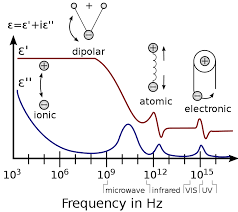
\includegraphics[width=0.8\columnwidth]{images/t1.png}
		\caption{Real and Imaginary part of permittivity (dielectric constant) as a function of frequency}
	\end{figure}
	
	\subsection{Variation of the dielectric constant\\
	in alternating fields}
		We are aware that an electric field causes a dielectric to become polarised. In a field that changes direction, the polarisation will likewise change direction to match the new field. The transfer of charges or the rotation of dipoles requires time, therefore this cannot happen instantly.

		The average dipole orientation adjusts over a particular period of time known as the relaxation time when the field is altered. 10 to 11 seconds are typical relaxing times. As a result, if the electric field alternates directions at a frequency greater than 1011 Hz, the polarization mechanism no longer contributes to the polarisation of the dielectric because the dipole orientation is unable to "keep up" with the alternating field and cannot maintain its alignment with it. The polarization process stops helping to polarise the dielectric at higher frequencies because the flow of charge cannot keep up with the alternating field. As frequency rises, the material's net polarisation decreases because it no longer contributes to the overall polarisation, and as a result, its dielectric constant decreases.

	\subsection{Variation of the dielectric constant in Temperature}
		The electrostatic forces generated by the field cause the molecules to rotate and align with it. However, due to the thermal motion the molecules are experiencing, not all of them are perfectly aligned with the field.

		Because the molecules have more thermal energy as the temperature rises, the amplitude of random thermal motion also increases. As a result, the molecules are less tightly aligned with one another, which results in less orientation polarisation of the material and a lower dielectric constant. This indicates that the range of departure from a perfect alignment with the external electric field is higher.

		As the temperature is reduced, the dielectric constant does not, however, rise continuously. At phase boundaries, the dielectric constant will abruptly alter. This is because during a phase transition, the structure alters, and as we've shown above, the structure has a significant impact on the dielectric constant.


	\subsection{$BaTiO^3$ Properties}

		Perovskite substance barium titanate has a relatively high dielectric constant at ambient temperature. the name of a group of substances that have the perovskite crystal structure, which is the same as that of calcium titanium oxide $(CaTiO_3)$. Perovskite has the following structure. While B-site cations sit in the centre of the body, A-site cations take up the corners of a cube. On the faces are three oxygen atoms per cell.

		\begin{figure}[H]
			\centering
			\label{fig:2}
			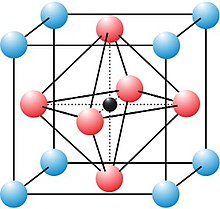
\includegraphics[width=0.4\columnwidth]{images/t3.jpg}
			\caption{Perovskite Structure}
		\end{figure}

		Below and beyond its $120^\circ C$ Curie point, barium titanate exhibits a paraelectric cubic phase and a ferroelectric tetragonal phase. The contaminants in a sample and the synthesis method have an impact on the Curie point temperature of that sample. In the paraelectric cubic phase, the centres of positive charges ($Ba^{2+}$, $Ti^{4+}$) coincide with the centres of negative charges ($O^{-2} ion$). However, when the temperature is cooled below Tc, we observe a tetragonal phase in which the centres of the $Ba^{2+}$ and $Ti^{4+}$ ions are dislocated in relation to the $O^{-2} ion$, resulting in the formation of electric dipoles. As a result, the of BaTiO3 rises until $T_c$ and reaches its maximum value at $T = T_c$ due to the divergence of susceptibility at that point.	After crossing this temperature it starts decreasing due to the formation of the cubic phase.

		\subsection{Study of diffuseness parameter}
  			The diffuseness parameter $\delta$ is defined as the slope of the log($\frac{1}{\epsilon}$ -$\frac{1}{\epsilon_c}$) vs log($\frac{1}{T}$ -$\frac{1}{T_c}$) plot where $\epsilon$ is the dielectric constant at a temperature T > $T_c$, ${\epsilon_c}$  is the maximum value of the dielectric constant at the Curie temperature $T_c$.  $\delta$ is expected to lie between 1 and 2.
